\documentclass{standalone}
\usepackage{tikz}
\begin{document}

\newcommand*\circled[1]{\tikz[baseline=(char.base)]{
            \node[shape=circle,draw] (char) {#1};}}

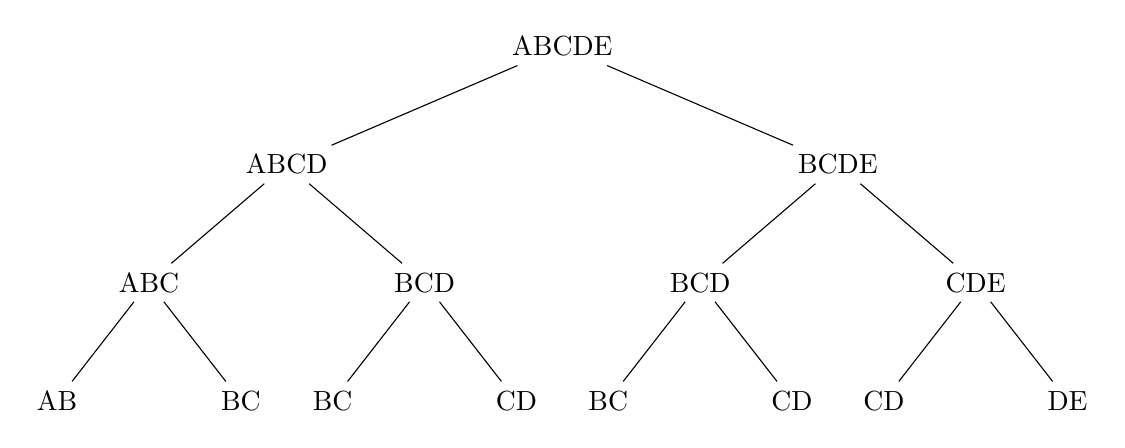
\begin{tikzpicture}[level/.style={sibling distance = 7cm/#1, level distance = 1.5cm}] 
	\begin{scope}[shift={(-6cm,0)}]
		\node (Root) {\circled{ABCDE}}
			child{ node{\circled{ABCD}}
			    child{ node{\circled{ABC}}
			            child{ node {\circled{AB}}}
			            child{ node {\circled{BC}}}  
			    }
			    child{ node {\circled{BCD}}
			            child{ node {\circled{BC}}}
			            child{ node {\circled{CD}}}
					}
				}
			child{ node{\circled{BCDE}}
			    child{ node{\circled{BCD}}
			            child{ node {\circled{BC}}}
			            child{ node {\circled{CD}}}  
			    }
			    child{ node {\circled{CDE}}
			            child{ node {\circled{CD}}}
			            child{ node {\circled{DE}}}
					}
				}				
		; 
	\end{scope}   
\end{tikzpicture}

\end{document}